\documentclass[12pt,a4paper]{article}
\usepackage[margin=2cm]{geometry}
\usepackage{xeCJK}
\usepackage{fontspec}
\setCJKmainfont{Noto Serif CJK TC}[Script=CJK]
\usepackage{amsmath,amssymb}
\usepackage{graphicx}
\usepackage{fancyhdr}
\setlength{\headheight}{14.5pt}
\addtolength{\topmargin}{-2.5pt}
\usepackage{hyperref}
\usepackage{listings}
\usepackage{enumitem}
\usepackage{titlesec}
\usepackage{caption}
\usepackage{indentfirst}
\usepackage{float}
\usepackage{forest}
\setlength{\parindent}{2em}
\pagestyle{fancy}
\fancyhf{}
\cfoot{\thepage}
\linespread{1.3}

\usepackage{multirow}
\usepackage{booktabs}   % 放在 preamble

% tikz tools for ER diagram
\usepackage{tikz}
\usetikzlibrary{shapes,positioning,calc}
\colorlet{lightgray}{gray!20}


\usepackage{minted}
\setminted{
    linenos,                % 行號
    frame=lines,            % 上下框線
    framesep=5pt,           % 程式碼與邊框距離
    numbersep=8pt,          % 行號與程式碼距離
    fontsize=\scriptsize,   % 字體大小
    breaklines,             % 自動換行
    tabsize=4,              % tab 寬度
    rulecolor=\color{black},% 框線顏色
    xleftmargin=1.5em       % 左側縮排
}


\title{資料庫管理 HW02}
\author{B12508026戴偉璿}
\date{}

\begin{document}

\maketitle

\lhead{資料庫管理 HW02}
\rhead{B12508026戴偉璿}

\begin{enumerate}
    \item
    \begin{enumerate}
        \item
        \begin{enumerate}
            \item \textbf{TRUE}, because \texttt{DEAN} is a \textbf{relation} between \texttt{COLLEGE} and \texttt{INSTRUCTOR}; and \texttt{CHAIR} is a \textbf{relation} between \texttt{DEPT} and \texttt{INSTRUCTOR}.
            \item \textbf{FALSE}, there's no further restriction on \texttt{DEAN} and \texttt{CHAIR}, so one \texttt{INSTRUCTOR} can be a \texttt{CHAIR} and a \texttt{DEAN} at the same time.
            \item \textbf{TRUE}, the relation between \texttt{STUDENT} and \texttt{HAS} is a \textbf{(0, 1)} relation, so one \texttt{STUDENT} can \texttt{HAS} zero or one \texttt{DEPT}.
            \item \textbf{TRUE}, the cardinality between \texttt{STUDENT} and \texttt{TAKES} is \textbf{(0, N)}, so one student may take zero or more sections; while the cardinality between \texttt{SECTION} and \texttt{TAKES} is \textbf{(5, N)}, so one section must be taken by five or more students.
            \item \textbf{TRUE}, the cardinality between \texttt{COURSE} and \texttt{SECTION} is \textbf{(1, 1)}, so one section must be related to exactly one course.
        \end{enumerate}
        \item As the following diagram:
        
        
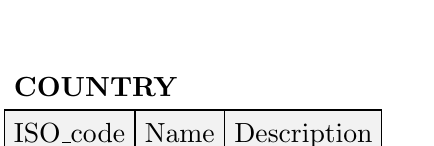
\begin{tikzpicture}[relation/.style={rectangle split, rectangle split parts=#1, rectangle split part align=base, draw, anchor=center, align=center, text height=3mm, text centered}]\hspace*{-0.3cm}

% RELATIONS

\node (countrytitle) {\textbf{COUNTRY}};

\node [relation=3, rectangle split horizontal, rectangle split part fill={lightgray!50}, anchor=north west, below=0.6cm of countrytitle.west, anchor=west] (INSTRUCTOR)
{\underline{ISO\_code}%
\nodepart{two}   Name
\nodepart{three} Description};


% FOREIGN KEYS



\end{tikzpicture}
    \end{enumerate}
 
\end{enumerate}



\end{document}